%% ----------------------------------------------------------------
%% Introduction.tex
%% ---------------------------------------------------------------- 
\chapter{Requirements and Analysis} \label{Chapter:three}

This chapter will analyse the requirements of the proposed application and inform the design decisions that have been made.

% \section{Technologies}
% \begin{itemize}
% \item{React}
% \item{Swagger}
% \item{Database}
% \item{Python}
% \item{Robot Framework}
% \end{itemize}
% [Insert functional requirements table here]
\section{Use cases}
Explanation

\begin{figure}[]
    \center
    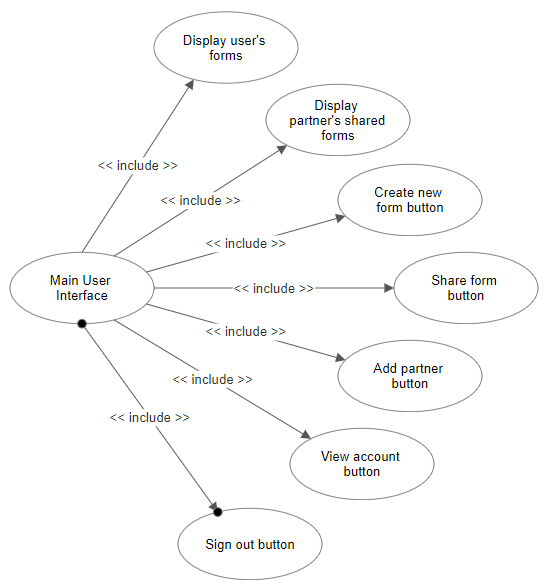
\includegraphics{../figures/UseCaseInterface}
    \caption{Use Case Diagram 1}
\end{figure}

\begin{figure}[]
    \center
    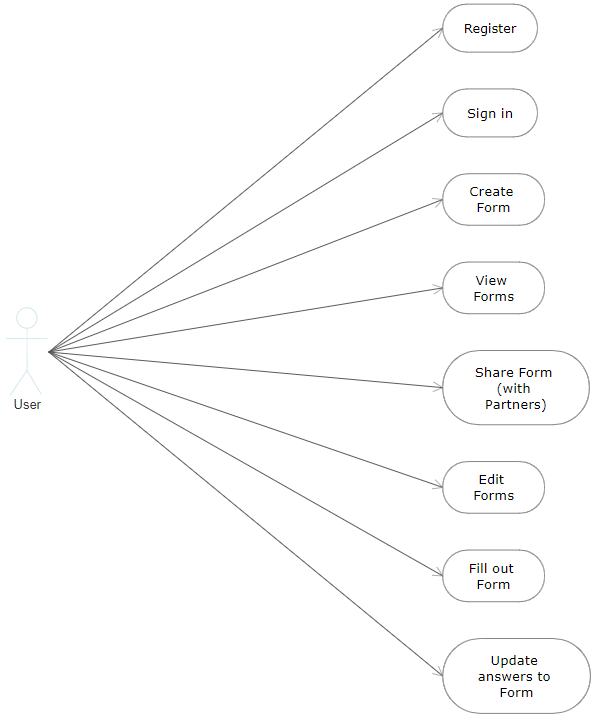
\includegraphics{../figures/UseCaseUser}
    \caption{Use Case Diagram 2}
\end{figure}

\subsection{Use case description}

The following table explains the main use cases of this project. (//TODO: CHANGE THIS LINE)

\begin{table}
    \centering
    \begin{tabular}{|c|c|}
        \hline
        Use Case & Description\\
        \hline
        \hline
        Display user's forms & A list of forms created by the user will be\\ & displayed, with the form's name, owner\\ & and date of last modification.\\
        \hline
        Display parter's shared form & A list of forms shared with the user by a partner\\ & will be displayed, with the form's name,\\ & owner and date of last modification.\\
        \hline
        Create new form button & Takes the user to a page where they can design a new form.\\
        \hline
        Share form button & Allows the user to share forms they have created with partners.\\
        \hline
        Add partner button & Allows the user to search for other people's accounts\\ & on the application, and add them as partners. This\\ & should be done with people you wish to share\\ & forms with or receive forms from.\\
        \hline
        View account button & Allows the user to view their account information\\ & and edit it if necessary. Details such\\ & as name, email, company and the ability\\ & to change the account's password.\\
        \hline
        Sign out button & Allows the user to sign out from the application.\\
        \hline
    \end{tabular}
    \caption{Use case descriptions}
    \label{tab:my_label}
\end{table}

\section{Functional requirements}
Explanation

\begin{table}
    \centering
    \begin{tabular}{|c|c|}
        \hline
        Requirement & Description\\
        \hline
        \hline
        Register & New users will create an account\\ & before being allowed to use the application\\
        \hline
        Log in & Users will need to log in before\\ & they are able to access their account, create,\\ & share and complete forms\\
        \hline
        Create a form & Users will be able to create a new\\ & form, which will be saved to their account\\
        \hline
        Share a form & users will be able to share a form\\ & that they have created with a partner\\
        \hline
        Add a partner & Users will be able to view and edit\\ & their account information, including; name,\\ & email, company and password(not viewable)\\
        \hline
        Sign out & Users will be able to sign out of the application\\
        \hline
        Notifications & Users will be notified of various changes, including\\ & their partners' answers to forms\\
        \hline
    \end{tabular}
    \caption{Functional requirements}
    \label{tab:my_label}
\end{table}

Requirements analysis table (Requirement(stated above) | Complexity | Time | Importance)

\section{Non-functional requirements}
Explanation\\table

\section{Risk analysis}
Explanation\\tables



\section{Functionality}

\begin{figure}[]
\center
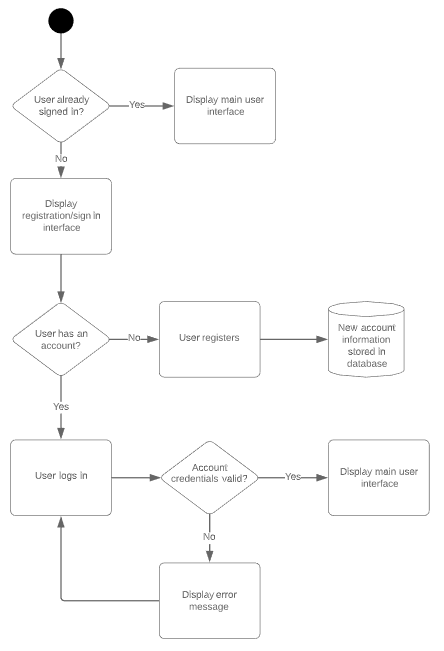
\includegraphics{../figures/ActivityDiagramAuthentication}
\caption{Activity Diagram: Authentication}
\end{figure}

\begin{figure}[]
\center
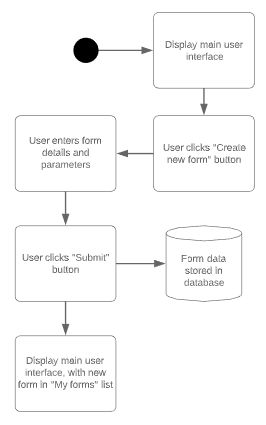
\includegraphics{../figures/ActivityDiagramFormCreation}
\caption{Activity Diagram: Form Creation}
\end{figure}

\begin{figure}[]
\center
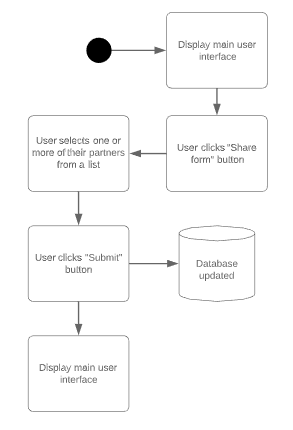
\includegraphics{../figures/ActivityDiagramFormSharing}
\caption{Activity Diagram: Form Sharing}
\end{figure}

\begin{figure}[]
\center
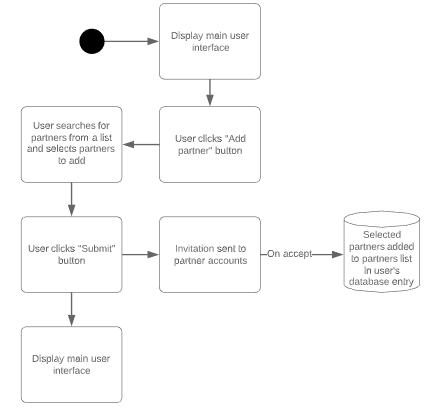
\includegraphics{../figures/ActivityDiagramPartnerInvitation}
\caption{Activity Diagram: Partner Invitation}
\end{figure}
